\documentclass[english,notitlepage]{revtex4-1}  % defines the basic parameters of the document
%For preview: skriv i terminal: latexmk -pdf -pvc filnavn



% if you want a single-column, remove reprint

% allows special characters (including æøå)
\usepackage[utf8]{inputenc}
%\usepackage[english]{babel}

%% note that you may need to download some of these packages manually, it depends on your setup.
%% I recommend downloading TeXMaker, because it includes a large library of the most common packages.

\usepackage{physics,amssymb}  % mathematical symbols (physics imports amsmath)
\include{amsmath}
\usepackage{graphicx}         % include graphics such as plots
\usepackage{xcolor}           % set colors
\usepackage{hyperref}         % automagic cross-referencing (this is GODLIKE)
\usepackage{listings}         % display code
\usepackage{subfigure}        % imports a lot of cool and useful figure commands
\usepackage{float}
%\usepackage[section]{placeins}
\usepackage{algorithm}
\usepackage[noend]{algpseudocode}
\usepackage{subfigure}
\usepackage{tikz}
\usetikzlibrary{quantikz}
% defines the color of hyperref objects
% Blending two colors:  blue!80!black  =  80% blue and 20% black
\hypersetup{ % this is just my personal choice, feel free to change things
    colorlinks,
    linkcolor={red!50!black},
    citecolor={blue!50!black},
    urlcolor={blue!80!black}}

%% Defines the style of the programming listing
%% This is actually my personal template, go ahead and change stuff if you want



%% USEFUL LINKS:
%%
%%   UiO LaTeX guides:        https://www.mn.uio.no/ifi/tjenester/it/hjelp/latex/
%%   mathematics:             https://en.wikibooks.org/wiki/LaTeX/Mathematics

%%   PHYSICS !                https://mirror.hmc.edu/ctan/macros/latex/contrib/physics/physics.pdf

%%   the basics of Tikz:       https://en.wikibooks.org/wiki/LaTeX/PGF/Tikz
%%   all the colors!:          https://en.wikibooks.org/wiki/LaTeX/Colors
%%   how to draw tables:       https://en.wikibooks.org/wiki/LaTeX/Tables
%%   code listing styles:      https://en.wikibooks.org/wiki/LaTeX/Source_Code_Listings
%%   \includegraphics          https://en.wikibooks.org/wiki/LaTeX/Importing_Graphics
%%   learn more about figures  https://en.wikibooks.org/wiki/LaTeX/Floats,_Figures_and_Captions
%%   automagic bibliography:   https://en.wikibooks.org/wiki/LaTeX/Bibliography_Management  (this one is kinda difficult the first time)
%%   REVTeX Guide:             http://www.physics.csbsju.edu/370/papers/Journal_Style_Manuals/auguide4-1.pdf
%%
%%   (this document is of class "revtex4-1", the REVTeX Guide explains how the class works)


%% CREATING THE .pdf FILE USING LINUX IN THE TERMINAL
%%
%% [terminal]$ pdflatex template.tex
%%
%% Run the command twice, always.
%% If you want to use \footnote, you need to run these commands (IN THIS SPECIFIC ORDER)
%%
%% [terminal]$ pdflatex template.tex
%% [terminal]$ bibtex template
%% [terminal]$ pdflatex template.tex
%% [terminal]$ pdflatex template.tex
%%
%% Don't ask me why, I don't know.

\begin{document}

\title{Project 2}      % self-explanatory
\author{Sverre Wehn Noremsaune \& Frida Marie Engøy Westby}          % self-explanatory
\date{\today}                             % self-explanatory
\noaffiliation                            % ignore this, but keep it.


\maketitle 
    
\begin{center}
	\url{https://github.uio.no/comPhys/FYS3150/tree/project2/project2}
\end{center}


\section*{Problem 1 - Second order differential equation}
In this problem we are looking at:

\begin{equation}
    \gamma \frac{d^2u(x)}{dx^2} = -Fu(x) \label{eq1}
\end{equation}

and 

\begin{equation}
    \frac{d^2 u(\hat{x})}{dx^2} = - \lambda u(\hat{x}) \label{eq2}
\end{equation}

We know from the assignment that $\hat{x} \equiv x/L \Rightarrow x = \hat{x}L$ and $\lambda = \frac{FL^2}{\gamma}$, and by appling this, we can see that (\ref{eq2}) is the scaled version of (\ref{eq1}): 

\begin{align*}
    \gamma \frac{d^2u(x)}{dx^2} &= -Fu(x)\\
    \frac{d^2u(x)}{dx^2} &= - \frac{Fu(x)}{\gamma}\\
\end{align*}

Put in $x = \hat{x}L$:

\begin{align*}
    \frac{d^2u(\hat{x}L)}{d(\hat{x}L)^2} &= - \frac{Fu(\hat{x}L)}{\gamma}\\
    \frac{d^2u(\hat{x})L}{d(\hat{x})^2L^2} &= - \frac{Fu(\hat{x})L}{\gamma}\\
\end{align*}

Then we multiplies both sides with $L$:

\begin{equation*}
    \frac{d^2u(\hat{x})L^2}{d(\hat{x})^2L^2} = - \frac{Fu(\hat{x})L^2}{\gamma}
\end{equation*}

Now we can use $\lambda = \frac{FL^2}{\gamma}$ and we easily see that we get (\ref{eq2}). $\blacksquare$


\section*{Problem 2 - Jacobi’s rotation algorithm}

From the assignment we have:

\begin{itemize}
    \item $\vec{v}_i$ is a set of orthonormal basis vectors: $\vec{v}_i^T \cdot \vec{v}_i = \delta_{ij}$
    \item $\mathbf{U}$ is an orthogonal transformation matrix: $\mathbf{U}^T = \mathbf{U}^{-1}$
\end{itemize}

From this we can show that tansformations with $\mathbf{U}$ preserves orthonormality, i.e. that $\vec{w}_i = \mathbf{U} \vec{v}_i$ will also be an orthonormal set:

\begin{equation*}
    \vec{w}_i^T \cdot \vec{w}_j = (\mathbf{U}\vec{v}_i)^T (\mathbf{U} \vec{v}_j) = \vec{v}_i^T \mathbf{U}^T \mathbf{U} \vec{v}_j = \vec{v}_i^T \mathbf{U}^{-1} \mathbf{U} \vec{v}_j 
    = \vec{v}_i^T  \mathbf{I} \vec{v}_j = \vec{v}_i^T  \cdot \vec{v}_j = \delta_{ij} \;\; \blacksquare
\end{equation*}


\section*{Problem 3 - The tridiagonal matrix $\mathbf{A}$}
See 'triag.cpp' for code and 'test\_triag.cpp' for test. 

\section*{Problem 4 - Largest off-diagonal element}

\subsection*{Problem a}
See 'max\_offdiag\_symmetric.cpp'.

\subsection*{Problem b}
See 'test\_max\_offdiag\_symmetric.cpp'.

\section*{Problem 5 - Implementation of Jacobi’s rotation }

\subsection*{Problem a}
See 'jacobi\_eigensolver.cpp'.

\subsection*{Problem b}
See 'test\_jacobi\_eigensolver.cpp'.

\section*{Problem 6 - Transformations}

\subsection*{Problem a}
See 'estimate\_rotations.cpp' and FIG \ref{transformations}.

\begin{figure}[H]
	\centering
	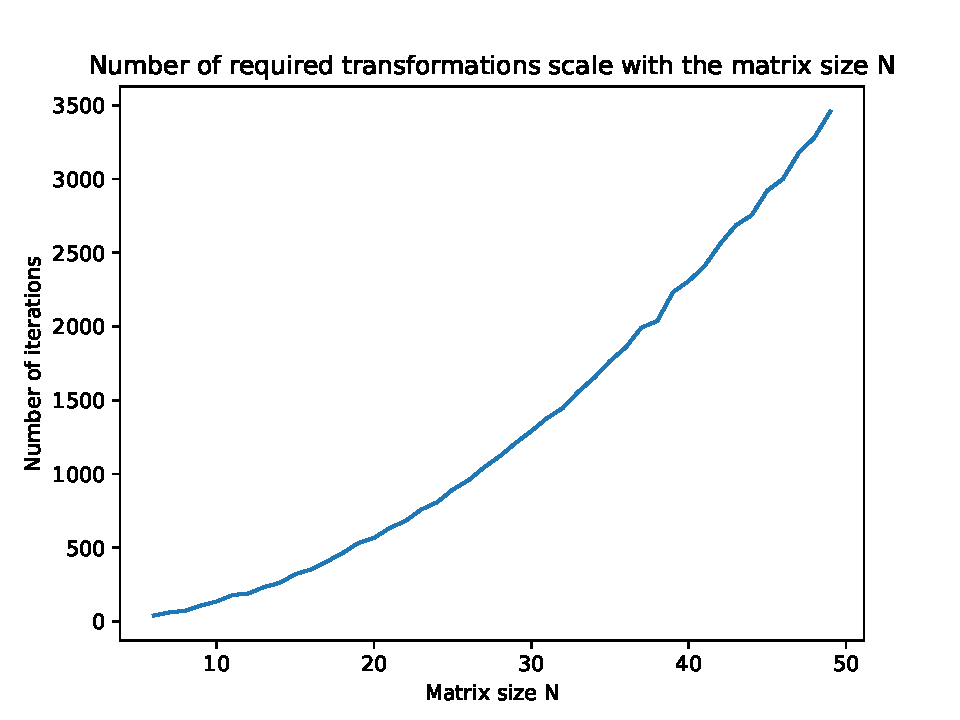
\includegraphics[scale=0.55]{plots/transformations.pdf} %Imports the figure.
	\caption{Number of required transformations scale with the tridiagonal matrix of size N}
	\label{transformations}
\end{figure}

\subsection*{Problem b}
The scaling behavior we expect to see if $\mathbf{A}$ was a dense matrix is that insted of having a $\mathcal{O}(n^2)$ we have $\mathcal{O}(n^3)$.


\section*{Problem 7 - Eigenvalue problem}

\subsection*{Problem a}
See 'solve\_diff.cpp' and FIG \ref{disc10}.

\begin{figure}[H]
	\centering
	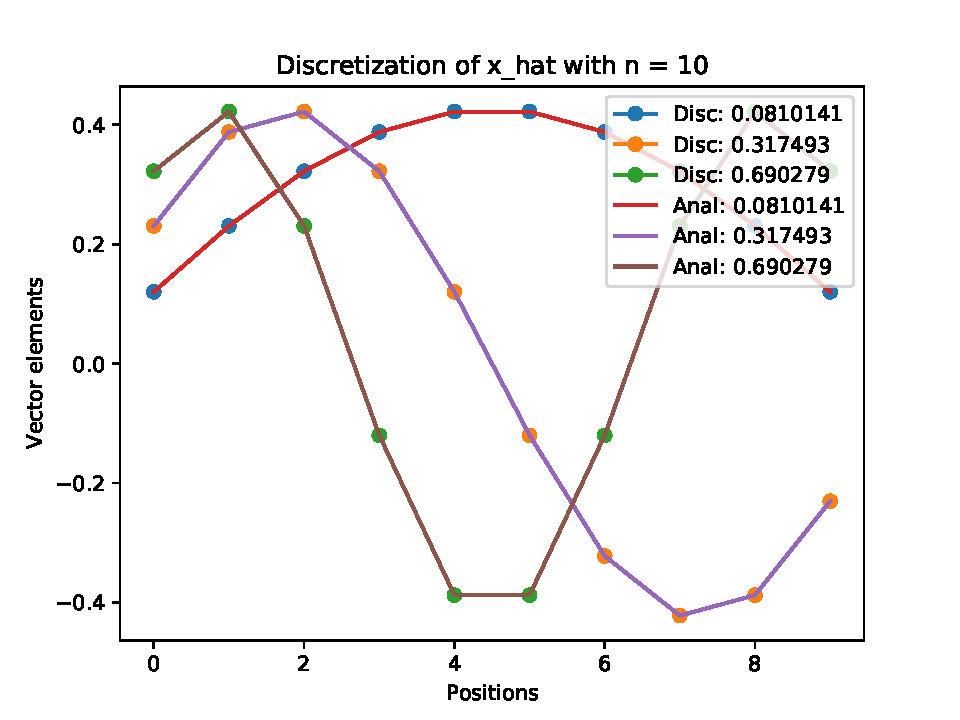
\includegraphics[scale=0.55]{plots/discretization_n10.pdf} %Imports the figure.
	\caption{Plot of the discrete eigenvectors the and corresponding analytical eigenvectors for N = 10}
	\label{disc10}
\end{figure}

\subsection*{Problem b}
See 'solve\_diff.cpp' and FIG \ref{disc100}.

\begin{figure}[H]
	\centering
	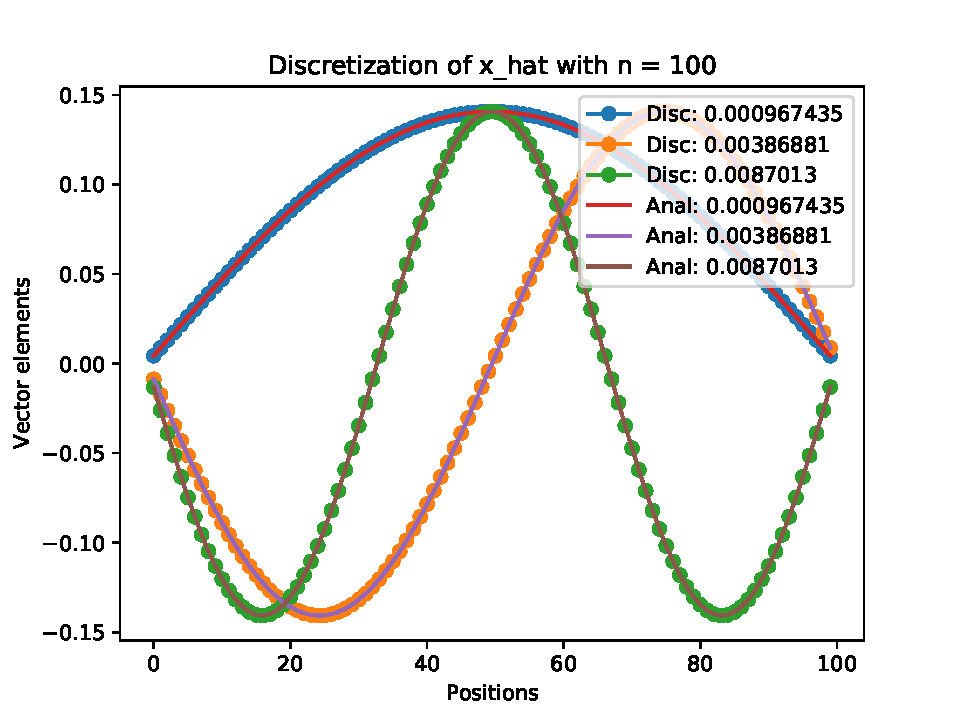
\includegraphics[scale=0.55]{plots/discretization_n100.pdf} %Imports the figure.
	\caption{Plot of the discrete eigenvectors the and corresponding analytical eigenvectors for N = 100}
	\label{disc100}
\end{figure}

\end{document}